% Used AI to help me decide on the flow of the theory chapter.
% This chapter gives the scientific background that justifies the design of the
% AIS‑anomaly visualisation prototype.  The layout follows a “lab‑process”
% pattern: domain → digital‑twin → visual‑analysis concepts → web‑mapping stack
% → rendering → software‑engineering foundations → agile development.

This chapter introduces

%=====================================================================
% 2.1  Automatic Identification System (AIS)
%=====================================================================
\section{Automatic Identification System (AIS)}
% source: Kystverket AIS‑Norway description (project brief)
The Automatic Identification System (AIS) is a system that transfers navigation data. However the system is prone to errors due to wrong configurations, area jamming, or message spoofing. Kystverket processes this data to detect errors in messages. In practice this pipeline identifies 60-80 million messages with errors every single day.
%=====================================================================
% 2.2  Digital Twin
%=====================================================================
\section{Digital Twin}
% source: IBM “What is a digital twin?” https://www.ibm.com/think/topics/digital-twin

A digital twin is a digital representation of a physical object or system. An AIS digital twin primarily represents a ship's location and speed, but it also stores additional information such as the vessel type. The main purpose of a digital twin is to enable real time tracking and to provide historical data for further analysis in the future if needed.
%   – economic and safety benefits are described in the Capgemini report .

%=====================================================================
% 2.3  Human‑Centric Data Visualisation
%=====================================================================
\section{Human‑Centric Data Visualisation}
% source: https://ieeexplore.ieee.org/document/5599750
Human visual perception excels at spotting patters and extracting meaningful information. However there are usually limits or systems that are harder for humans to recognize. Therefore, visualisation techniques focus on presenting data in a way that leverage's a humans pattern recognition.

\subsection{Heat‑Map Visualisation}
% source: https://www.atlassian.com/data/charts/heatmap-complete-guide
Heat-maps visualise point density with color gradients usually with warm to cold gradients. This system enables human operators to locate "hot-spots" of data. This is useful since human operators get a better visual distinction of areas compared to other visualisation methods such as scatter maps.


\subsection{Clustering}
% source: https://link.springer.com/article/10.1007/s12530-012-9062-5
Dynamic clustering adapts to the zoom level of the user by aggregating nearby points. This can cause 1 thousand points to become represented by 1 point labelled with 1000, which improves scale perception.

\subsection{Scatter Map (Geographic Scatter‑Plot)}
% source: https://www.atlassian.com/data/charts/what-is-a-scatter-plot
A scatter map plots individual AIS pings using latitude and longitude to provide a precice location once clusters are decomposed. When combined with clustering it perserves point accuracy while still conveying scale.

%=====================================================================
% 2.4  Web‑Mapping Stack
%=====================================================================
\section{Web‑Mapping Stack}
% source: https://doc.arcgis.com/en/arcgis-online/reference/what-is-web-map.htm
A web map is an interactive display composed of a map system, a rendering library, and a data-retrieval system. Its primary function is to present geographic information in a way that supports analysis.

\subsection{Vector Tiles}
% source: https://en.wikipedia.org/wiki/Vector_tiles
Vector tiles are packets of geographic data which are packaged into pre-defined square tiles. This hybrid approach maintains high visual quality while avoiding full map pre-rendering.

\subsection{MapLibre}
% source: https://maplibre.org/maplibre-gl-js/docs/  https://maplibre.org/maplibre-gl-js/docs/API/classes/Map/
Maplibre leverage's vector tiles and WebGL to render interactive maps directly in a browser. 

\subsection{REST API}
% source: https://www.redhat.com/en/topics/api/what-is-a-rest-api
The REST API provides AIS anomalies as GeoJSON files on request.

%=====================================================================
% 2.5  Rendering Acceleration
%=====================================================================
\section{Rendering Acceleration}
% source: https://www.geeksforgeeks.org/data-science/what-is-gpu-acceleration/
GPU-based hardware acceleration markedly improves the performance of compute-intensive applications. The principal uses of GPU's are graphics rendering and parallel computation.


\subsection{WebGL}
% source: https://en.wikipedia.org/wiki/WebGL
WebGL connects the GPU to the browser and allows Maplibre to render vector maps, when compared to the normal speed when using the cpu the result becomes fast enough that it seems real time.

%=====================================================================
% 2.6  Software‑Engineering Principles Might be in method unsure though.
%=====================================================================



%=====================================================================
% 2.7  Agile Development Practices Unsure if this should be here or in method.
%=====================================================================


%%%%%%%%%%%%%%%%%%%%%%%%%%%%%%%%%%%%%%%%%%%%%%%%%%%%%%%
%%%%%%%%%%%%%%%
%%%%%%%%%%%%%%%%
%%%%%%%%%%%%%%%%%%%


\begin{comment}

\section{Data visualization}
\noindent Processing massive datasets manually is inefficient, so data-visualisation techniques are required. Data visualization displays raw data in forms that leverage human perception to identify patterns, trends, and outliers. In the project we employ methods such as heatmaps and clusters, which intuitively display density with color gradients and aggregations of points.
https://www.ibm.com/think/topics/data-visualization
https://www.tableau.com/learn/articles/data-visualization


\subsection{Clustering}
Clustering pertains to a method of aggregating data points into groups or clusters. While clustering can be done based on specific parameters(like media genres or user details), in a geographic context, algorithms typically group objects based on density and proximity. Visualising large geographic datasets can easily cause visual clutter if thousands of individual data points are rendered in close proximity. Clustering can mitigate this by aggregating nearby data points into a single point/group based on the current zoom level of the map. As the user zooms in, the clusters will dynamically break apart into smaller groups or individual points. 
https://www.ibm.com/think/topics/clustering
https://developers.google.com/machine-learning/clustering/overview

\begin{figure}[H]
  \centering
  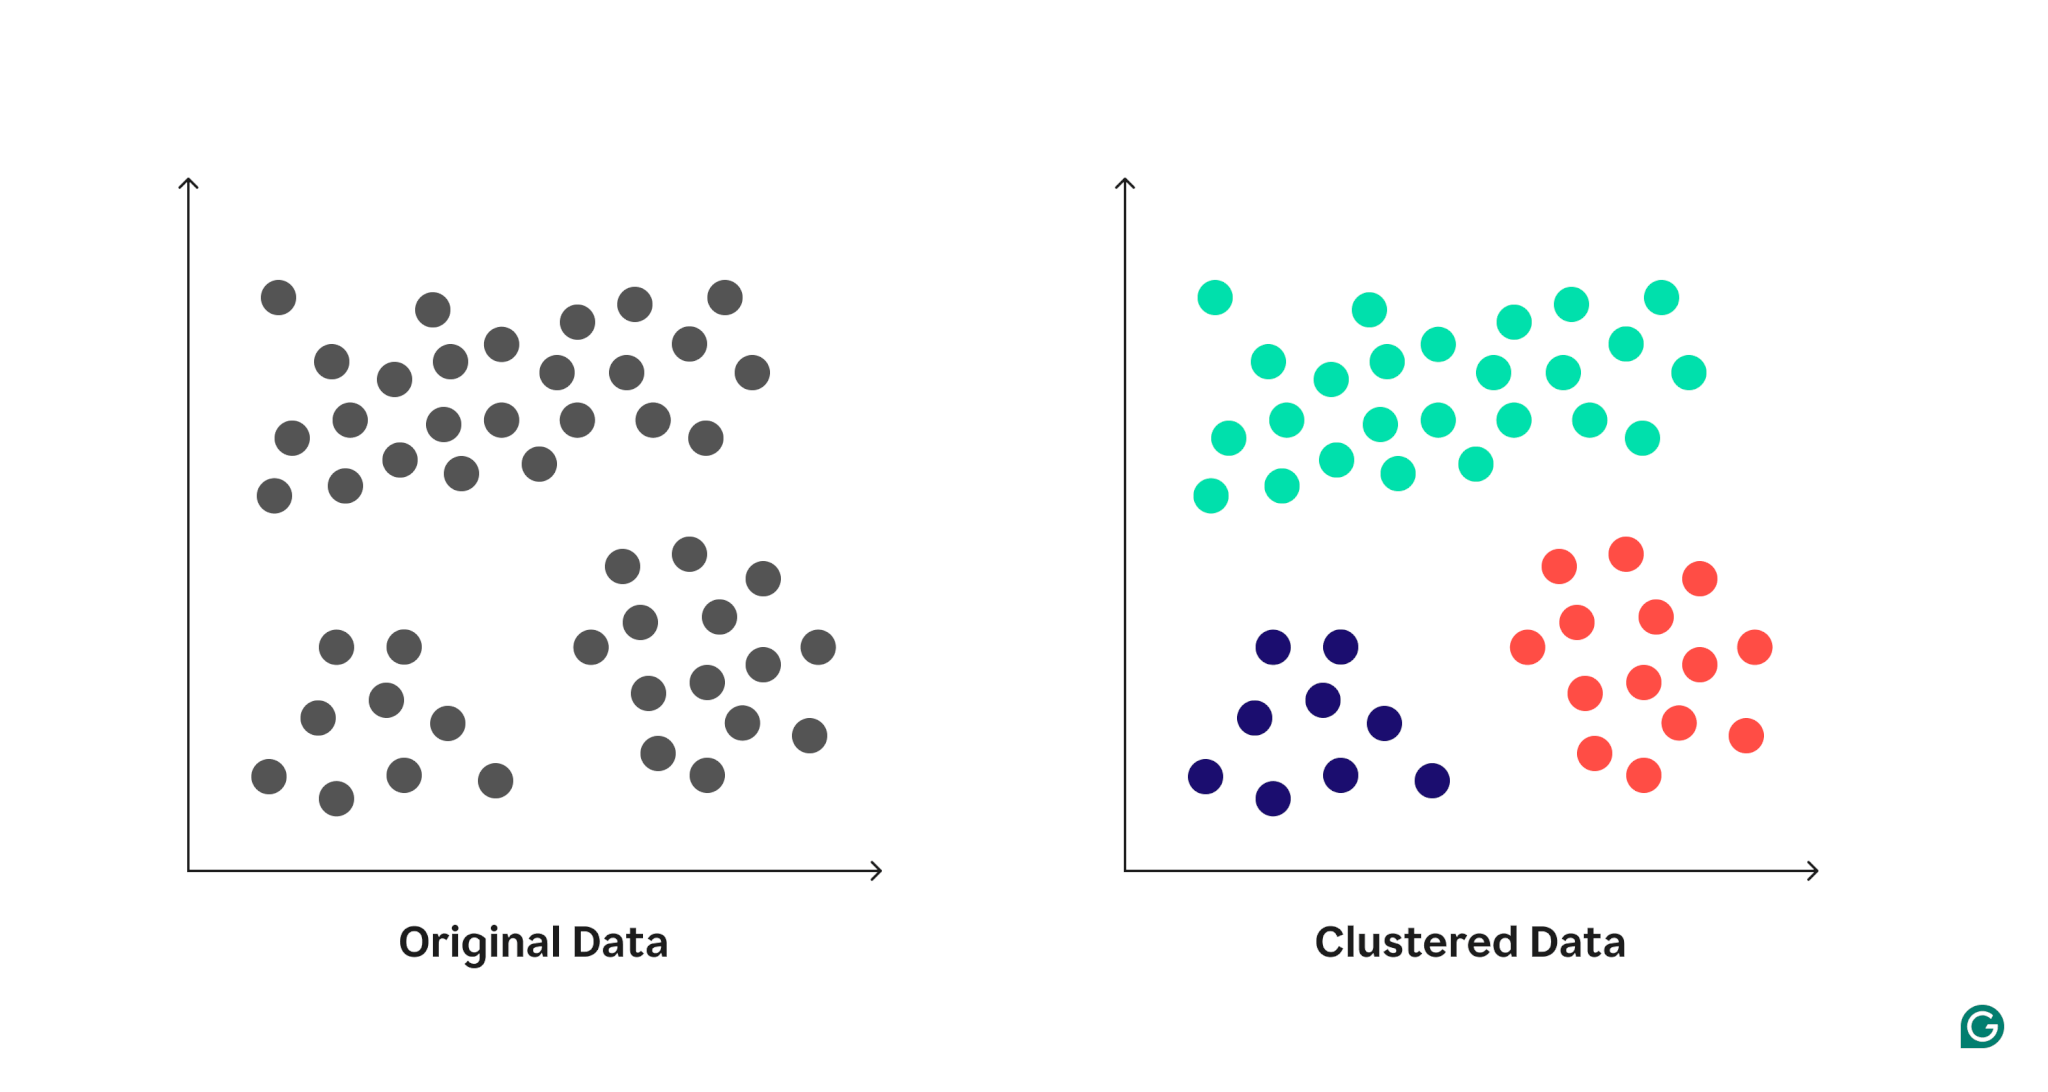
\includegraphics[width=0.9\textwidth]{Figures/Clustering_Data.png}
  \caption[Illustration of spatial data clustering]{Illustration of clustering of data points based on spatial proximity. Source: \url{https://www.grammarly.com/blog/ai/what-is-clustering/}}
  \label{fig:latlong}
\end{figure}


\subsection{Heat Map}
While clustering groups discrete points together, heat maps are used for data visualization to show relationship between variables and the density of data over a given area. The amount of data dictates a color gradient, leading to a higher concentration of data having a darker or warmer color than less concentrated areas. This leads to intuitive visualization of data for humans to parse, instantly highlighting "hotspots" of activity without needing to process individual data points. 
https://www.atlassian.com/data/charts/heatmap-complete-guide


\subsection{Scatter map}
A scatter map is a spatial adoption of a traditional scatter plot. Wherein a standard scatter plot is used to show correlation between variables on an abstract  x,y coordinate plane using statistical methods, a scatter map preforms this plotting using geographic coordinates. Each point of data is plotted using logitude as the X-axis and latitude as the Y-axis. This gives the user precise visualization of individual entities or incidents on a geographic map once a user zooms past the aggregated clustering layers.
https://www.atlassian.com/data/charts/what-is-a-scatter-plot

\section{Web Map}
Web maps are maps created for geographic visualization on the internet. They are a modern tool that allows users to have interactable maps on websites that are easy to use and insightful for what data is shown. Web maps are constructed by having a "basemap", which is the first layer showing the map itself without specific data. On top of the basemap, additional operational layers are added. This can be data points of incidents happening in a geographic area, charting of train tracks in a country, and much more that is defined by the needs of the user. 
https://www.mapbox.com/insights/web-maps


\subsection{vector tiles}
Vector tiles are the current standard utilized by most web map providers. Instead of the static PNG images that were used in the past, vector tiles save geographic data in a mathematical vector format. They allow for significantly more styling and customization than image-based formats, and have led to smoother, pixel-free zooming. However, because the browser must render the map geometry mathematically whenever the user zooms, this smoother usage comes at the cost of more processing power needed on the client's device.
https://docs.mapbox.com/data/tilesets/guides/vector-tiles-introduction/

\subsection{MapLibre}

\section{API}
In modern software architecture, an Application Programming Interface (API) is a crucial tool that allows communication between distinct software systems. In geographic applications, API's decouple the frontend web map from the from the backend database. So when a user interacts with the map, the frontend request specific subsets of data from the API, which returns the geographic coordinates in  a lightweight format such as JSON or GeoJSON.
https://aws.amazon.com/what-is/api/

\section{hardware acceleration}
Hardware acceleration is a method to get increased performance in computing tasks, which include rendering graphics and vector tiles in browsers. Hardware acceleration works by offloading tasks that are normally done by the CPU(Central Processing Unit) to other hardware in the computer like the GPU(Graphics Processing Unit). The GPU has massively more parallel processing capability than the CPU, significantly speeding up such computations for tasks that require it.
https://www.sciencedirect.com/topics/computer-science/hardware-acceleration

\subsection{WebGL}
In web enviorments, this hardware acceleration is achived via WebGL (Web Graphics Library).
\url{https://developer.mozilla.org/en-US/docs/Web/API/WebGL_API}


\section{Software principles}
To ensure that the software developed for this project remains scalable, maintainable, and robust, several core software engineering principles were adhered to. 

\subsection{Cohesion and Coupling}

\subsection{Testing}
lorem ipsum
lorem ipsum
lorem ipsum

\section{Agile Development}
This project was managed using Agile development principles. The Agile work flow prioritize adaptability, iterative progress, and continuous delivery. Which makes them ideal for software projects where technical requirements may evolve.
\subsection{Scrum and Issue Tracking}
lorem ipsum
lorem ipsum
lorem ipsum

%equations, bib. \\
%\section{Sprint/Scrum}
% Might make sprint its own section
\end{comment}
\begin{comment}
\section{Equations}

A simple equation can be included as: \\

\begin{equation}
        r = 2\pi^{2}
        \label{eqn:simple_eqn}
\end{equation} \\


\noindent The text below shows an example of how to align equations on the equal sign, with only one reference for both. This may be useful for when they are linked and are actually only one equation but splitting them up makes it more readable. \\

\begin{equation}
\begin{aligned}
        a &= \sin^{2}(\Delta\phi/2) + \cos(\phi_{1})\cdot\cos(\phi_{2})\cdot\sin^{2}(\Delta\lambda/2)\\
        d &= 2R\cdot\arcsin(\sqrt{a})
\end{aligned}
\label{eqn:haversine}
\end{equation} \\

\noindent The whole equation can be referenced as "equation \eqref{eqn:haversine}", here showing the Haversine formula. One may also align sub-equations such that they are numbered the same but have a letter differentiating them as shown below. This can be used when they are linked, but you will need to reference both individual parts.

\begin{subequations}
\begin{align}
    SSD 
        & \quad = \sum_{i=1}^{n} (\vec{x_{i}}-\vec{\mu_{q}})^{2} \label{eq:ssd}\\[15pt] %creates more space between the sub-equations
    SSE 
        & \quad = \sum_{q=1}^{k} \delta_{rq} SSD \label{eq:sse}
\end{align}
\label{eqn:subeqn}
\end{subequations} \\

\noindent These equations can be refrenced by their spesific sub-equation as "equation \eqref{eq:ssd}", or by the whole group as "equations \eqref{eqn:subeqn}". The "double backslashes" in the .tex creates line spaces and gives more room around the equations and paragraphs. Use them as you think feels right. 



\section{Tables and footnotes}

Here is an example of both a regular table with data and a table with split headers, for scientific usage. Do not use horizontal/vertical rulers between the data, or encase the table with rulers. \\

\begin{table}[ht!]
\centering
    \begin{tabular}{ m{3cm} m{2.5cm} m{2.5cm} m{2.5cm} m{2cm} } 
    \toprule
    \toprule
    \textbf{Statistic} & \textbf{Velocity} & \textbf{Altitude} & \textbf{1/Angle} & \textbf{Temp.} \\
    \midrule
    Mean    & 122.68    & 240.98   & 93.75     & 13.95 \\[1.3ex]
    Std     & 224.51    & 145.88   & 60.39     & 4.44  \\[1.3ex]
    Q1      & 28.00     & 111.60   & 34.15     & 10.60 \\[1.3ex]
    Median  & 63.00     & 223.20   & 99.59     & 13.30 \\[1.3ex]
    Q3      & 137.00    & 359.10   & 151.99    & 16.70 \\[1.3ex]
    Min     & 0.00      & 1.00     & 0.00      & 3.30  \\[1.3ex]
    Max     & 14519.00  & 616.70   & 180.00    & 32.10 \\[1.3ex]
    \bottomrule
    \bottomrule
    \end{tabular}
% the square brackets after \caption gives the table a proper title in the list of tables, instead of just inserting the beginning of the table caption
\caption[Dynamic feature statistics with outliers]{Table of dynamic feature statistics where outliers are included, for all data points. Velocity is given in \textit{m/h}, the altitude in \textit{mamsl}, the inverse trajectory angle in 1/degrees, and temperature in degrees Celsius.}
\label{table:stat_fliers}
\end{table}


\begin{table}[ht!]
\centering
    \begin{tabular}{ m{3cm} m{5cm} m{3cm} } 
    \toprule
    \toprule
    \textbf{Area 1} & \textbf{Start date} & \textbf{End date} \\
    \midrule
    2018    & 03.06    & 29.06                       \\[1.3ex]
    2019    & 03.06    & 03.07 or 31.08\footnotemark \\[1.3ex]
    2020    & 03.06    & 05.09                       \\[1.3ex]
    \midrule
    \textbf{Area 2} & \textbf{Start date (farm 1/2)} & \textbf{End date} \\
    \midrule
    2012    & 09.06            & 07.09               \\[1.3ex]
    2013    & 23.06 / 15.06    & 25.08               \\[1.3ex]
    2014    & 05.06 / 25.06    & 10.09               \\[1.3ex]
    2015    & 13.06 / 03.07    & 06.09               \\[1.3ex]
    2016    & 17.06            & 22.07               \\[1.3ex]
    \bottomrule
    \bottomrule
    \end{tabular}
\caption[Selected time ranges for all data]{Selected time ranges for the data in all areas and all years.}
\label{table:time_ranges}
\end{table}

\footnotetext{A footnote explaining something.}



\section{A single figure}

Figure \ref{fig:latlong} is included as an example. The square brackets before the caption description contains the title of the figure, which is what will be written in the list of figures. This should be short and concise. The same layout applies to tables and other floats. Remember to change the title as well as the caption if you are copying these examples. In the list of figures and tables all the different floats will be grouped together by chapter. Remember to always reference all your figures and tables in the text at least once.

\begin{figure}[H]
  \centering
  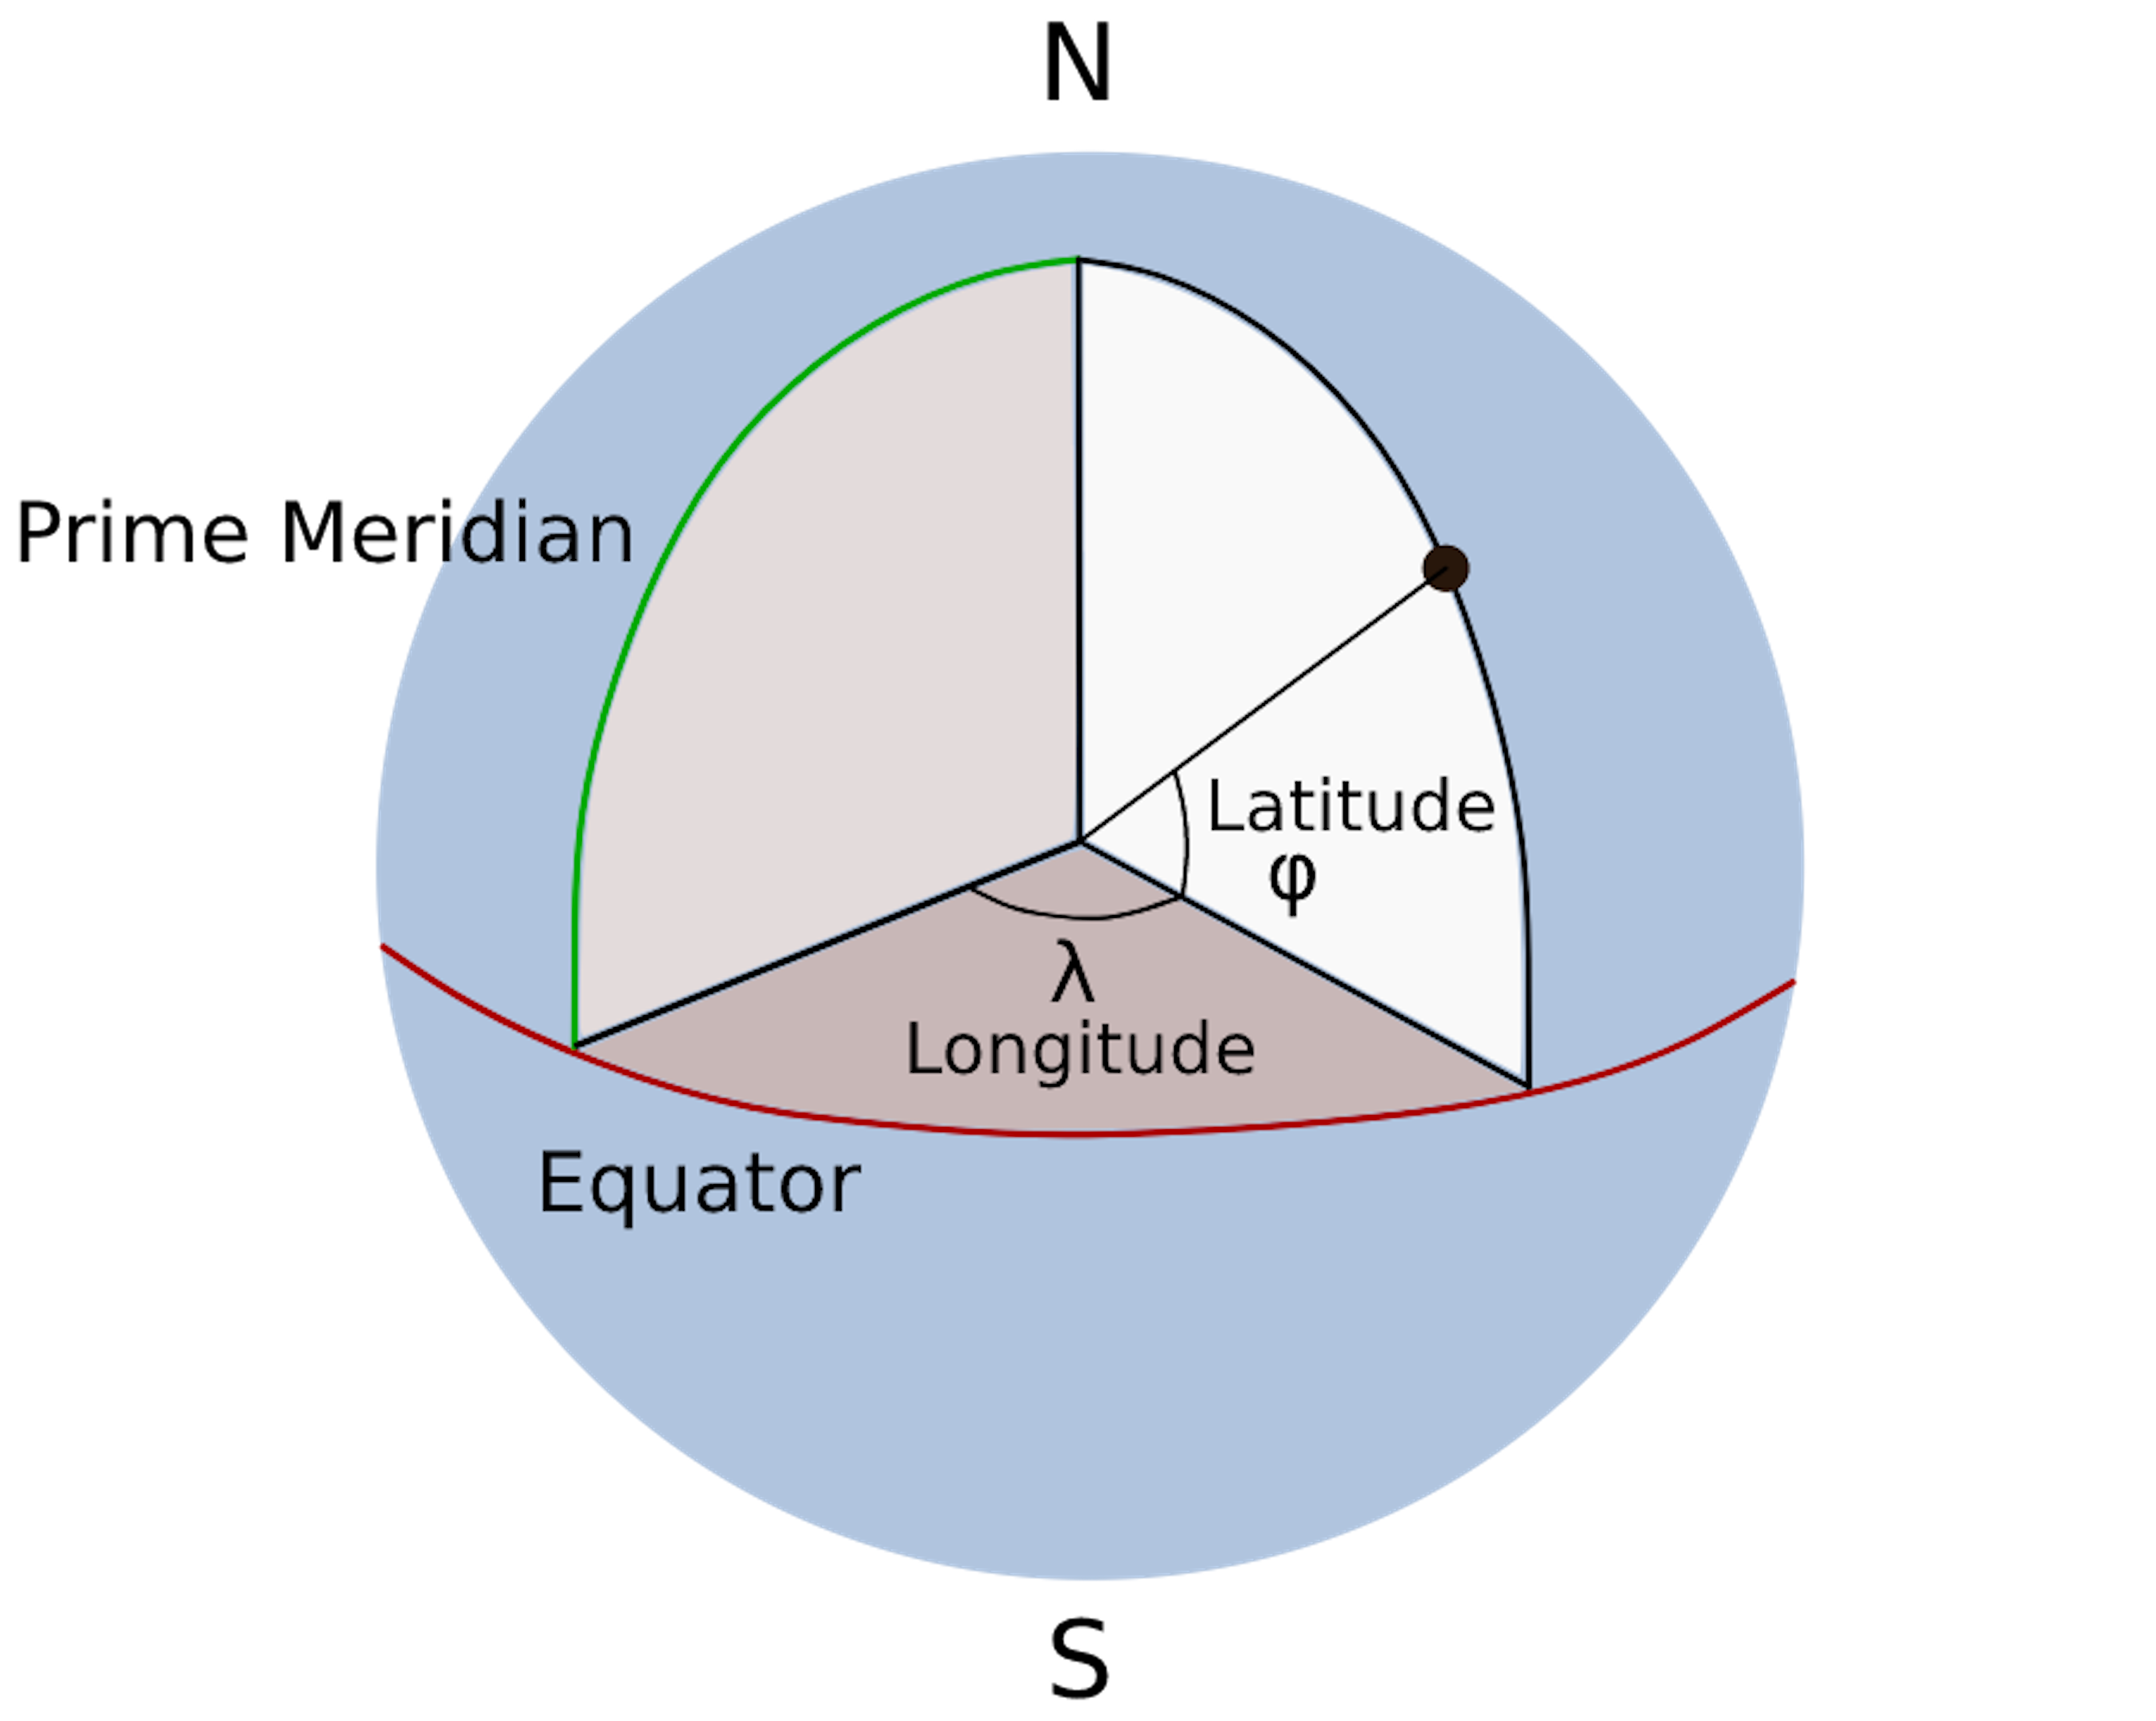
\includegraphics[width=0.9\textwidth]{Figures/latlong.png}
  \caption[Illustration of latitude and longitude]{Illustration of the earth, and how latitudes and longitudes are calculated with respect to the equator and the prime meridian.}
  \label{fig:latlong}
\end{figure}


\section{Citations}

Here are some examples on how to reference a source (where none is relevant to the text but just for illustration purposes only). One may cite a single reference by calling \cite{wolves_of_mount_mckinley}, or several in the same bracket by calling \cite{machine_learning, clustering_impossibility} when they are all related to the same statement. There are many different styles on how to cite, and how the layout and order of your citation style is presented. This is my favorite, as I find it neat and tidy \cite{sheep}. It will show up in order of appearance in the references section.
\end{comment}